\documentclass[12pt]{article}

% Opening
\title{Applied Combinatorics Homework 2}
\author{Akash Narayanan}
\usepackage{amsmath, amsfonts, amssymb, amsthm, enumitem, tikz}
\usepackage{caption, subcaption, float}

% Problem environment
\theoremstyle{definition}
\newtheorem{problem-internal}{Problem}[]
\newenvironment{problem}{
  \medskip
  \begin{problem-internal}
}{
\end{problem-internal}
}

% Solution environment
\newenvironment{solution}{
  \begin{proof}[Solution]
    \vspace{-8px}
    \setlength{\parskip}{4px}
    \setlength{\parindent}{0px}
}{
\end{proof}
}

\begin{document}

  \maketitle

  % Problem 1
  \begin{problem}
    Let \(N\) denote the set of positive integers. When \(f : N \rightarrow N \), let \(E(f)\) be the function defined by \(E(f)(n) = 2^{f(n)}\). What is \(E^{5}(n^2)\)?
  \end{problem}

  \begin{solution}
    A simple calculation shows that the function is
    \begin{align*}
      2^{2^{2^{2^{2^{n^{2}}}}}}
    \end{align*}
    which looks very ugly. It grows very quickly and would be an incredibly slow running time for an algorithm.
  \end{solution}

  % Problem 2
  \begin{problem}
    The questions in this exercise pertain to the graph \textbf{G} shown below.

    \begin{figure}[ht]
      \centering
      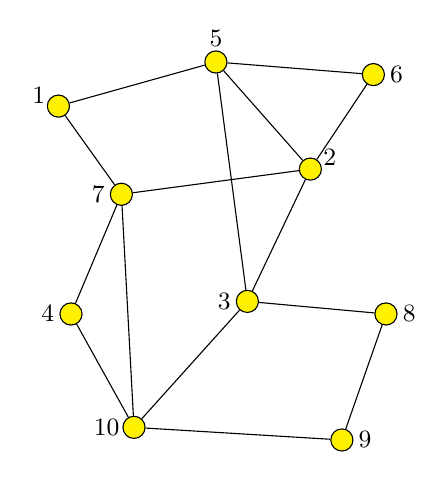
\begin{tikzpicture}
        [scale=0.8,every node/.style={draw,shape=circle,fill=yellow,inner sep=0,minimum size=8pt}]

        \node[label=170:{\small 1}] (v1) at (1, 5.3) {};
        \node[label=15:{\small 2}] (v2) at (5, 4.3) {};
        \node[label=left:{\small 3}] (v3) at (4, 2.2) {};
        \node[label=left:{\small 4}] (v4) at (1.2, 2) {};
        \node[label=above:{\small 5}] (v5) at (3.5, 6) {};
        \node[label=right:{\small 6}] (v6) at (6, 5.8) {};
        \node[label=left:{\small 7}] (v7) at (2, 3.9) {};
        \node[label=right:{\small 8}] (v8) at (6.2, 2) {};
        \node[label=right:{\small 9}] (v9) at (5.5, 0) {};
        \node[label=left:{\small 10}] (v10) at (2.2, 0.2) {};

        \draw (v1) -- (v5);
        \draw (v1) -- (v7);
        \draw (v2) -- (v3);
        \draw (v2) -- (v5);
        \draw (v2) -- (v6);
        \draw (v2) -- (v7);
        \draw (v3) -- (v5);
        \draw (v3) -- (v8);
        \draw (v3) -- (v10);
        \draw (v4) -- (v7);
        \draw (v4) -- (v10);
        \draw (v5) -- (v6);
        \draw (v7) -- (v10);
        \draw (v8) -- (v9);
        \draw (v9) -- (v10);
      \end{tikzpicture}
  \end{figure}

  \begin{enumerate}[label={\alph*.}]
    \item What is the degree of vertex 8?
    \item What is the degree of vertex 10?
    \item How many vertices of degree 2 are there in \textbf{G}? List them.
    \item Find a cycle of length 8 in \textbf{G}.
    \item What is the length of a shortest path from 3 to 4?
    \item What is the length of a shortest path from 8 to 7?
    \item Find a path of length 5 from vertex 4 to vertex 6.
  \end{enumerate}
  \hfill
  \end{problem}

  \begin{solution}
    \hfill
    \begin{enumerate}[label={\alph*.}]
      \item The degree of vertex 8 is 2.
      \item The degree of vertex 10 is 4.
      \item There are 5 vertices of degree 2. They are \(\{1, 4, 6, 8, 9\}\).
      \item A cycle of size 8 is \(1, 7, 4, 10, 9, 8, 3, 5\).
      \item A shortest path from 3 to 4 has size 3. It is \(3, 10, 4\).
      \item A shortest path from 8 to 7 has size 4. It is \(8, 9, 10, 7\).
      \item A path of size 5 from vertex 4 to vertex 6 is \(4, 10, 7, 2, 6\).
    \end{enumerate}
  \end{solution}

  % Problem 3
  \begin{problem}
    Draw a graph with 8 vertices, all of odd degree, that does not contain a path of length 3 or explain why such a graph does not exist.
  \end{problem}

  \begin{solution}
    \hfill
    \begin{figure}[H]
      \centering

      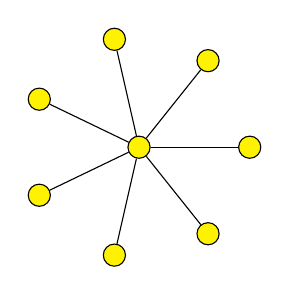
\begin{tikzpicture}
        [scale=1,every node/.style={draw,shape=circle,fill=yellow,inner sep=0,minimum size=8pt}]

        \node (1) at (0, 0) {};
        \node (2) at (360/7 * 0:40pt) {};
        \node (3) at (360/7 * 1:40pt) {};
        \node (4) at (360/7 * 2:40pt) {};
        \node (5) at (360/7 * 3:40pt) {};
        \node (6) at (360/7 * 4:40pt) {};
        \node (7) at (360/7 * 5:40pt) {};
        \node (8) at (360/7 * 6:40pt) {};

        \draw (1) -- (2);
        \draw (1) -- (3);
        \draw (1) -- (4);
        \draw (1) -- (5);
        \draw (1) -- (6);
        \draw (1) -- (7);
        \draw (1) -- (8);
      \end{tikzpicture}
    \end{figure}
  \end{solution}

  % Problem 4
  \begin{problem}
    Prove that every tree on \(n\) vertices has exactly \(n-1\) edges.
  \end{problem}

  \begin{solution}
    We prove the statement by induction on the number of vertices. For the base case of \(n=2\), the requirement that the graph be connected forces there to be exactly 1 edge between the two vertices. That is, \(n-1=1\) so the statement holds for 2 vertices.

    Now suppose the statement holds for \(n=k\) for some \(k \geq 2\). Consider a tree \textbf{T} with \(k+1\) vertices. We use the fact that every tree with 2 or more vertices has at least two leaves since by definition it has no cycles. We can remove a leaf and consider the remaining graph \textbf{T}\('\) with \(k\) vertices. Since the degree of a leaf is 1, the \textbf{T}\('\) has exactly one less edge than \textbf{T}. By the induction hypothesis, \textbf{T}\('\) has \(k-1\) edges. Then \textbf{T} has \(k\) edges. Indeed, \((k + 1) - 1 = k\) so the statement holds for \(n=k+1\). It can also be seen trivially that the statement holds for \(n=1\). By the Principle of Induction, the statement holds for all \(n \geq 1\).
  \end{solution}
  % \pagebreak
  % Problem 5
  \begin{problem}
    The figure below contains four graphs on six vertices. Determine which (if any) pairs of graphs are isomorphic. For pairs that are isomorphic, give an isomorphism between the two graphs. For pairs that are not isomorphic, explain why.

    \begin{figure}[H]
      \begin{subfigure}[b]{.49\textwidth}
        \centering

        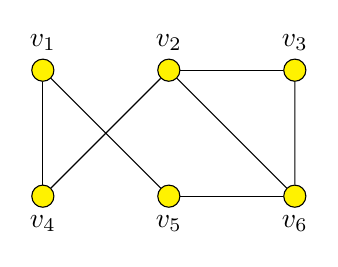
\begin{tikzpicture}
          [scale=0.8,every node/.style={draw,shape=circle,fill=yellow,inner sep=0pt,minimum size=8pt}]

          \node[label=90:{\(v_1\)}] (v1) at (0, 2) {};
          \node[label=90:{\(v_2\)}] (v2) at (2, 2) {};
          \node[label=90:{\(v_3\)}] (v3) at (4, 2) {};
          \node[label=270:{\(v_4\)}] (v4) at (0, 0) {};
          \node[label=270:{\(v_5\)}] (v5) at (2, 0) {};
          \node[label=270:{\(v_6\)}] (v6) at (4, 0) {};

          \draw (v1) -- (v5);
          \draw (v1) -- (v4);
          \draw (v2) -- (v3);
          \draw (v2) -- (v4);
          \draw (v2) -- (v6);
          \draw (v3) -- (v6);
          \draw (v5) -- (v6);
        \end{tikzpicture}
        \caption*{\textbf{G}\textsubscript{1}}
      \end{subfigure}
      \hspace*{3pt}
      \begin{subfigure}[b]{.49\textwidth}
        \centering

        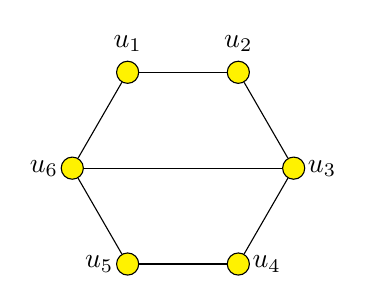
\begin{tikzpicture}
          [scale=1,every node/.style={draw,shape=circle,fill=yellow,inner sep=0pt,minimum size=8pt}]

          \node[label=90:{\(u_1\)}] (u1) at (120:40pt) {};
          \node[label=90:{\(u_2\)}] (u2) at (60:40pt) {};
          \node[label=0:{\(u_3\)}] (u3) at (0:40pt) {};
          \node[label=0:{\(u_4\)}] (u4) at (300:40pt) {};
          \node[label=180:{\(u_5\)}] (u5) at (240:40pt) {};
          \node[label=180:{\(u_6\)}] (u6) at (180:40pt) {};

          \draw (u1) -- (u2);
          \draw (u1) -- (u6);
          \draw (u2) -- (u3);
          \draw (u3) -- (u4);
          \draw (u3) -- (u6);
          \draw (u4) -- (u5);
          \draw (u5) -- (u6);
        \end{tikzpicture}
        \caption*{\textbf{G}\textsubscript{2}}
      \end{subfigure}

      \bigskip

      \begin{subfigure}[b]{.49\textwidth}
        \centering

        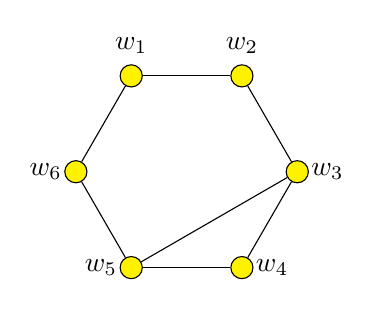
\begin{tikzpicture}
          [scale=1,every node/.style={draw,shape=circle,fill=yellow,inner sep=0pt,minimum size=8pt}]

          \node[label=90:{\(w_1\)}] (w1) at (120:40pt) {};
          \node[label=90:{\(w_2\)}] (w2) at (60:40pt) {};
          \node[label=0:{\(w_3\)}] (w3) at (0:40pt) {};
          \node[label=0:{\(w_4\)}] (w4) at (300:40pt) {};
          \node[label=180:{\(w_5\)}] (w5) at (240:40pt) {};
          \node[label=180:{\(w_6\)}] (w6) at (180:40pt) {};

          \draw (w1) -- (w2);
          \draw (w1) -- (w6);
          \draw (w2) -- (w3);
          \draw (w3) -- (w4);
          \draw (w3) -- (w5);
          \draw (w4) -- (w5);
          \draw (w5) -- (w6);
        \end{tikzpicture}
        \caption*{\textbf{G}\textsubscript{3}}
      \end{subfigure}
      \hspace*{3pt}
      \begin{subfigure}[b]{.49\textwidth}
        \centering

        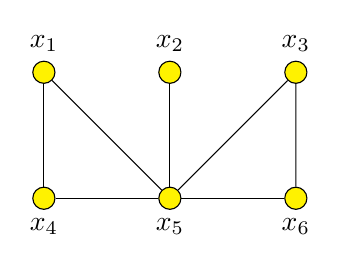
\begin{tikzpicture}
          [scale=0.8,every node/.style={draw,shape=circle,fill=yellow,inner sep=0pt,minimum size=8pt}]

          \node[label=90:{\(x_1\)}] (x1) at (0, 2) {};
          \node[label=90:{\(x_2\)}] (x2) at (2, 2) {};
          \node[label=90:{\(x_3\)}] (x3) at (4, 2) {};
          \node[label=270:{\(x_4\)}] (x4) at (0, 0) {};
          \node[label=270:{\(x_5\)}] (x5) at (2, 0) {};
          \node[label=270:{\(x_6\)}] (x6) at (4, 0) {};

          \draw (x1) -- (x4);
          \draw (x1) -- (x5);
          \draw (x2) -- (x5);
          \draw (x3) -- (x5);
          \draw (x3) -- (x6);
          \draw (x4) -- (x5);
          \draw (x5) -- (x6);
        \end{tikzpicture}
        \caption*{\textbf{G}\textsubscript{4}}
      \end{subfigure}
    \end{figure}
  \end{problem}

  \begin{solution}
    \textbf{G}\textsubscript{1} and \textbf{G}\textsubscript{2} are not isomorphic. This can be seen by noting that \textbf{G}\textsubscript{1} has a cycle of size 3 whereas the smallest cycle in \textbf{G}\textsubscript{2} is of size 4.

    \textbf{G}\textsubscript{1} is isomorphic to \textbf{G}\textsubscript{3}. Let \(\phi\) be a bijective map from \textbf{V}\textsubscript{1} to \textbf{V}\textsubscript{2} defined as follows
    \begin{align*}
      \phi(v_1) = w_1
      \quad
      \phi(v_2) = w_3
      \quad
      \phi(v_3) = w_4 \\
      \phi(v_4) = w_2
      \quad
      \phi(v_5) = w_6
      \quad
      \phi(v_6) = w_5
    \end{align*}
    It can easily be verified that this bijection is in fact a graph isomorphism.

    Since \textbf{G}\textsubscript{3} is isomorphic to \textbf{G}\textsubscript{1}, which is not isomorphic to \textbf{G}\textsubscript{2}, it follows that \textbf{G}\textsubscript{3} is not isomorphic to \textbf{G}\textsubscript{2}.

    Finally, neither \textbf{G}\textsubscript{1}, \textbf{G}\textsubscript{2}, nor \textbf{G}\textsubscript{3} is isomorphic to \textbf{G}\textsubscript{4} because the fourth graph contains a vertex of degree 1, which none of the other graphs contain.
  \end{solution}

  % Problem 6
  \begin{problem}
    Explain why the graph \textbf{G} below does not have an eulerian circuit, but show that by adding a single edge, you can make it eulerian.

    \begin{figure}[ht]
      \centering
      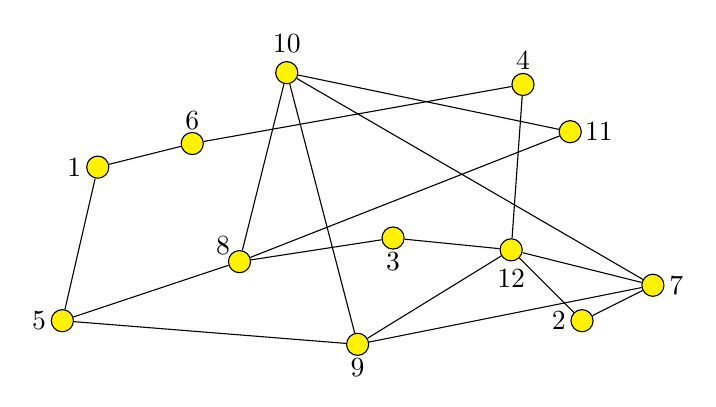
\begin{tikzpicture}
        [scale=1.5,every node/.style={draw,shape=circle,fill=yellow,inner sep=0,minimum size=8pt}]

        \node[label=180:{1}] (v1) at (0, 0) {};
        \node[label=180:{2}] (v2) at (4.1, -1.3) {};
        \node[label=270:{3}] (v3) at (2.5, -0.6) {};
        \node[label=90:{4}] (v4) at (3.6, 0.7) {};
        \node[label=180:{5}] (v5) at (-0.3, -1.3) {};
        \node[label=90:{6}] (v6) at (0.8, 0.2) {};
        \node[label=0:{7}] (v7) at (4.7, -1) {};
        \node[label=135:{8}] (v8) at (1.2, -0.8) {};
        \node[label=270:{9}] (v9) at (2.2, -1.5) {};
        \node[label=90:{10}] (v10) at (1.6, 0.8) {};
        \node[label=0:{11}] (v11) at (4, 0.3) {};
        \node[label=270:{12}] (v12) at (3.5, -0.7) {};

        \draw (v1) -- (v5);
        \draw (v1) -- (v6);
        \draw (v2) -- (v7);
        \draw (v2) -- (v12);
        \draw (v3) -- (v8);
        \draw (v3) -- (v12);
        \draw (v4) -- (v6);
        \draw (v4) -- (v12);
        \draw (v5) -- (v8);
        \draw (v5) -- (v9);
        \draw (v7) -- (v9);
        \draw (v7) -- (v10);
        \draw (v7) -- (v12);
        \draw (v8) -- (v10);
        \draw (v8) -- (v11);
        \draw (v9) -- (v10);
        \draw (v9) -- (v12);
        \draw (v10) -- (v11);
      \end{tikzpicture}
    \end{figure}
  \end{problem}

  \begin{solution}
    The graph does not have an eulerian circuit because it has vertices of odd degree, namely 5 and 12. This means that not every edge can be traversed exactly once since a cycle wouldn't be able to enter and exit that vertex. The conclusion follows from Euler's Theorem. However, this can be fixed by adding an edge between vertices 5 and 12. This changes the graph so that every vertex has even degree. One eulerian circuit on this new graph would be (1, 5, 9, 10, 8, 11, 10, 7, 12, 9, 7, 2, 12, 5, 8, 3, 12, 4, 6)
  \end{solution}

  % Problem 7
  \begin{problem}
    Find the chromatic number of the graph \textbf{G} shown below and a coloring using \(\chi\)(\textbf{G}) colors.

    \begin{figure}[H]
      \centering

      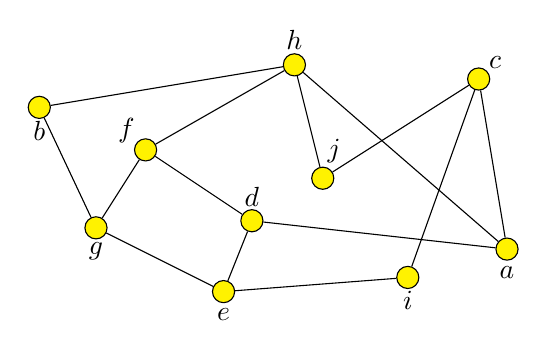
\begin{tikzpicture}
        [scale=1.8,every node/.style={draw,shape=circle,fill=yellow,inner sep=0, minimum size=8pt}]

        \node[label=270:{\(a\)}] (a) at (1.3, -0.5) {};
        \node[label=270:{\(b\)}] (b) at (-2, 0.5) {};
        \node[label=45:{\(c\)}] (c) at (1.1, 0.7) {};
        \node[label=90:{\(d\)}] (d) at (-0.5, -0.3) {};
        \node[label=270:{\(e\)}] (e) at (-0.7, -0.8) {};
        \node[label=135:{\(f\)}] (f) at (-1.25, 0.2) {};
        \node[label=270:{\(g\)}] (g) at (-1.6, -0.35) {};
        \node[label=90:{\(h\)}] (h) at (-0.2, 0.8) {};
        \node[label=270:{\(i\)}] (i) at (0.6, -0.7) {};
        \node[label={[label distance=2pt]85:{\(j\)}}] (j) at (0, 0) {};

        \draw (a) -- (c);
        \draw (a) -- (d);
        \draw (a) -- (h);
        \draw (b) -- (g);
        \draw (b) -- (h);
        \draw (c) -- (i);
        \draw (c) -- (j);
        \draw (d) -- (e);
        \draw (d) -- (f);
        \draw (e) -- (g);
        \draw (e) -- (i);
        \draw (f) -- (g);
        \draw (f) -- (h);
        \draw (h) -- (j);
      \end{tikzpicture}
    \end{figure}
  \end{problem}

  \begin{solution}
    The chromatic number of this graph \(\chi (\textbf{G}) = 3\). The chromatic number is greater than 2 since the graph contains a cycle of odd length, namely \(\left(a, c, i, e, d \right)\). A 3-coloring might partition the vertex set as follows: \(\{\{a, e, f, j\}, \{b, i\}, \{c, d, g, h\}\}\). A visualization of such a coloring is given below.

    \begin{figure}[ht]
      \centering

      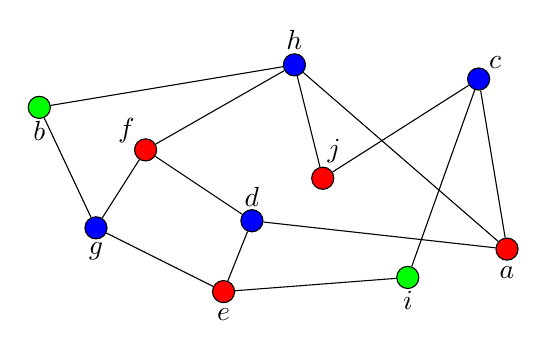
\begin{tikzpicture}
        [scale=1.8,every node/.style={draw,shape=circle,inner sep=0, minimum size=8pt}]

        \node[label=270:{\(a\)},fill=red] (a) at (1.3, -0.5) {};
        \node[label=270:{\(b\)},fill=green] (b) at (-2, 0.5) {};
        \node[label=45:{\(c\)},fill=blue] (c) at (1.1, 0.7) {};
        \node[label=90:{\(d\)},fill=blue] (d) at (-0.5, -0.3) {};
        \node[label=270:{\(e\)},fill=red] (e) at (-0.7, -0.8) {};
        \node[label=135:{\(f\)},fill=red] (f) at (-1.25, 0.2) {};
        \node[label=270:{\(g\)},fill=blue] (g) at (-1.6, -0.35) {};
        \node[label=90:{\(h\)},fill=blue] (h) at (-0.2, 0.8) {};
        \node[label=270:{\(i\)},fill=green] (i) at (0.6, -0.7) {};
        \node[label={[label distance=2pt]85:{\(j\)}},fill=red] (j) at (0, 0) {};

        \draw (a) -- (c);
        \draw (a) -- (d);
        \draw (a) -- (h);
        \draw (b) -- (g);
        \draw (b) -- (h);
        \draw (c) -- (i);
        \draw (c) -- (j);
        \draw (d) -- (e);
        \draw (d) -- (f);
        \draw (e) -- (g);
        \draw (e) -- (i);
        \draw (f) -- (g);
        \draw (f) -- (h);
        \draw (h) -- (j);
      \end{tikzpicture}
    \end{figure}
  \end{solution}

\end{document}
